%% Artikelvorlage unter Verwendung der Artikelklasse des KOMA-Script %%
%% Basierend auf einer TeXNicCenter-Vorlage von Mark M�ller          %%
%%%%%%%%%%%%%%%%%%%%%%%%%%%%%%%%%%%%%%%%%%%%%%%%%%%%%%%%%%%%%%%%%%%%%%%

% W�hlen Sie die Optionen aus, indem Sie % vor der Option entfernen  
% Dokumentation des KOMA-Script-Packets: scrguide

%%%%%%%%%%%%%%%%%%%%%%%%%%%%%%%%%%%%%%%%%%%%%%%%%%%%%%%%%%%%%%%%%%%%%%%
%% Optionen zum Layout des Artikels                                  %%
%%%%%%%%%%%%%%%%%%%%%%%%%%%%%%%%%%%%%%%%%%%%%%%%%%%%%%%%%%%%%%%%%%%%%%%
\documentclass[%
%a5paper,							% alle weiteren Papierformat einstellbar
%landscape,						% Querformat
10pt,								% Schriftgr��e (12pt, 11pt (Standard))
%BCOR1cm,							% Bindekorrektur, bspw. 1 cm
%DIVcalc,							% f�hrt die Satzspiegelberechnung neu aus
%											  s. scrguide 2.4
%twoside,							% Doppelseiten
%twocolumn,						% zweispaltiger Satz
%halfparskip*,				% Absatzformatierung s. scrguide 3.1
%headsepline,					% Trennline zum Seitenkopf	
%footsepline,					% Trennline zum Seitenfu�
%titlepage,						% Titelei auf eigener Seite
%normalheadings,			% �berschriften etwas kleiner (smallheadings)
%idxtotoc,						% Index im Inhaltsverzeichnis
%liststotoc,					% Abb.- und Tab.verzeichnis im Inhalt
%bibtotoc,						% Literaturverzeichnis im Inhalt
%abstracton,					% �berschrift �ber der Zusammenfassung an	
%leqno,   						% Nummerierung von Gleichungen links
%fleqn,								% Ausgabe von Gleichungen linksb�ndig
%draft								% �berlangen Zeilen in Ausgabe gekennzeichnet
]
{article}


% Seiten-Gr��e einstellen ist mit dem Geometry-Package viel einfacher
%  a4paper                DIN A4-Papier
%  text={width,height}    gibt H�he und Breite des Text-Bereiches an
%  centering              zentriert den Textbereich auf der Seite
%  landscape|portrait     Quer-/Hochformat
\usepackage[a4paper,text={160mm,255mm},centering,headsep=5mm,footskip=10mm]{geometry}

%\pagestyle{empty}		% keine Kopf und Fu�zeile (k. Seitenzahl)
%\pagestyle{headings}	% lebender Kolumnentitel  


%% Fonts f�r pdfLaTeX, falls keine cm-super-Fonts installiert %%%%%%%%
%\ifpdf
	%\usepackage{ae}        % Benutzen Sie nur
	%\usepackage{zefonts}  	% eines dieser Pakete
%\else
	%%Normales LaTeX - keine speziellen Fontpackages notwendig
%\fi

%% optischer Randausgleich, falls pdflatex verwandt %%%%%%%%%%%%%%%%%%%
\usepackage[activate]{pdfcprot}				

%% Packages f�r Grafiken & Abbildungen %%%%%%%%%%%%%%%%%%%%%%
\usepackage{graphicx} %%Grafiken in pdfLaTeX
%\usepackage[hang]{subfigure} %%Mehrere Teilabbildungen in einer Abbildung
%\usepackage{pst-all} %%PSTricks - nicht verwendbar mit pdfLaTeX

%% deutsche Anpassung %%%%%%%%%%%%%%%%%%%%%%%%%%%%%%%%%%%%%%%%%%%%%%%%%
\usepackage[english]{babel}		
\usepackage[T1]{fontenc}							
\usepackage[latin1]{inputenc}		

\usepackage{color}
\usepackage{hyperref}
\definecolor{darkblue}{rgb}{0,0,0.3}
\definecolor{darkgreen}{rgb}{0,.3,0}
\definecolor{darkred}{rgb}{.3,0,0}
\hypersetup{pdftex=true,citecolor=black,colorlinks=true,breaklinks=true,linkcolor=black,menucolor=black,pagecolor=black,urlcolor=black}

\usepackage{amsmath}
\usepackage{longtable}
\usepackage{ifsym}
\usepackage{float}


\begin{document}
%% Dateiendungen f�r Grafiken %%%%%%%%%%%%%%%%%%%%%%%%%%%%%%%
%% ==> Sie k�nnen hiermit die Dateiendung einer Grafik weglassen.
%% ==> Aus "\includegraphics{titel.eps}" wird "\includegraphics{titel}".
%% ==> Wenn Sie nunmehr 2 inhaltsgleiche Grafiken "titel.eps" und
%% ==> "titel.pdf" erstellen, wird jeweils nur die Grafik eingebunden,
%% ==> die von ihrem Compiler verarbeitet werden kann.
%% ==> pdfLaTeX benutzt "titel.pdf". LaTeX benutzt "titel.eps".
\ifpdf
	\DeclareGraphicsExtensions{.pdf,.jpg,.png}
\else
	\DeclareGraphicsExtensions{.eps}
\fi

\pagestyle{empty} %%Keine Kopf-/Fusszeilen auf den ersten Seiten.


%%%%%%%%%%%%%%%%%%%%%%%%%%%%%%%%%%%%%%%%%%%%%%%%%%%%%%%%%%%%%%%%%%%%%%%
%% Ihr Artikel                                                       %%
%%%%%%%%%%%%%%%%%%%%%%%%%%%%%%%%%%%%%%%%%%%%%%%%%%%%%%%%%%%%%%%%%%%%%%%

%% eigene Titelseitengestaltung %%%%%%%%%%%%%%%%%%%%%%%%%%%%%%%%%%%%%%%    
%\begin{titlepage}
%Einsetzen der TXC Vorlage "Deckblatt" m�glich
%\end{titlepage}

%% Angaben zur Standardformatierung des Titels %%%%%%%%%%%%%%%%%%%%%%%%
%\titlehead{Titelkopf }
%\subject{Typisierung}
\title{Cobolt Laser Remote Control}
\author{Jan Krieger <j.krieger@dkfz.de> / <jan@jkrieger.de>\footnote{German Cancer Research Center (DKFZ), Department: Biophysics of Macromolecules (Prof. J. Langowski), Im Neuenheimer Feld 580, D-69120 Heidelberg, Germany, tel: +49-6221/42-3395}}
%\and{Der Name des Co-Autoren}
%\thanks{Elisabeth Brama, now @ University of Sussex, Brighton}			% entspr. \footnote im Flie�text
%\date{}							% falls anderes, als das aktuelle gew�nscht
%\publishers{Herausgeber}

%% Widmungsseite %%%%%%%%%%%%%%%%%%%%%%%%%%%%%%%%%%%%%%%%%%%%%%%%%%%%%%
%\dedication{Widmung}

\maketitle 						% Titelei wird erzeugt

%% Zusammenfassung nach Titel, vor Inhaltsverzeichnis %%%%%%%%%%%%%%%%%
%\begin{abstract}
% F�r eine kurze Zusammenfassung des folgenden Artikels.
% F�r die �berschrift s. \documentclass[abstracton].
%\end{abstract}

%% Erzeugung von Verzeichnissen %%%%%%%%%%%%%%%%%%%%%%%%%%%%%%%%%%%%%%%
\tableofcontents			% Inhaltsverzeichnis
%\listoftables				% Tabellenverzeichnis
%\listoffigures				% Abbildungsverzeichnis


%% Der Text %%%%%%%%%%%%%%%%%%%%%%%%%%%%%%%%%%%%%%%%%%%%%%%%%%%%%%%%%%%
\newpage
\section{Introduction}
\label{sec:Introduction}
This circuit implements a remote control for Cobolt Generation 4 Laser controllers. It was designed due to the lack of a simple means to regulate laser power on the above mentioned laser without a Computer connected to them. Basically this remote control consists of a small microcontroller which communicates with the laser controller. A small liquid-crystal display is connected, so the user may read the current laser status and error information. A rotary encoder knob allows to set the desired laser power. In addition this circuit implements a USB interface for the connection to a PC and thus allows also remote control from there. Figure~\ref{fig:overview} shows an overview of the system and the cabling.

\begin{figure}[H]
	\centering
		\includegraphics{overview.pdf}
	\caption{Overview and Cabling of Cobolt laser together with remote control box}
	\label{fig:overview}
\end{figure}

In addition to the basic functionality described above, the interface also features four auxiliary I/Os that may be read/set by the user, if the interface is connected to a PC. Two of these lines may also be used to control the laser with external voltages. In the \textit{external on/off mode} a TTL-Input line (3,3V levels!) replaces the 0/1 push button. In the \textit{external intensity mode} a second line may be used to set the laser power by applying a voltage between 0 and 2.56V. The response is linear here. For details see section \ref{sec:ExternalControlModes}.

The following section \ref{sec:Usage} explains how to operate the control box. Then section \ref{sec:Realization} will give a detailed description of the system and explain the implementation. In section \ref{sec:USBInterfaceCommandReference} the USB interface to the PC will be explained and a command reference is given.

\newpage
\section{Wiring of the Control Box}
\label{sec:WiringOfTheControlBox}
The wiring of the control box is quite simple. In the simplest mode of operation you will need a 5V wall plug (e.g. SPS 2500-5 from Voltcraft) that fits into the second connector from left (diameter of center pin: 1.3mm, diameter of opening 4.5mm, 5V is connected to center pin, GND to the outer contact). Note that you may destroy the control box with a wrong polarity (to be fixed in future versions). Then you will have to connect the interface to the laser using a standard USB-Mini-B to USB-A connector.

If you also need a connection of the control box to the PC, you may connect a USB-A/B cable to the USB connector on the right-hand side and the PC. The auxiliary I/O are available on a 2x3 pinhead connector block with 2.54mm pin distance.


\section{Usage}
\label{sec:Usage}
This section describes the basic operation of the remote control box. Figure~\ref{fig:panel} shows the control panel. The user interacts by use of these elements:
\begin{itemize}
	\item a 3 line \textbf{liquid crystal display (LCD)}, shows the current state and available options.
	\item a \textbf{rotary encoder (RE)}, which also features a push button (REB) that allows to set the laser power in normal operations mode and the different parameters in the configuration mode
	\item an \textbf{on/off button (OOB)}, which allows to switch the laser on and off in normal operations mode. This button is back illuminated to indicate the actual on/off state of the laser.
	\item a \textbf{menu button (MB)}, which allows to change from normal operation mode to the configuration menu.
	\item a green \textbf{laser power LED (LPLED)}, which indicates whether the laser is connected or not
	\item a red \textbf{error LED (ELED)}, which indicates any error state. If this is on, an error message should appear in the second line of the LCD
	\item a yellow \textbf{lock LED (LLED)}, which indicates whether the laser lock works properly.
\end{itemize}
\begin{figure}[H]
	\centering
		\includegraphics{panel.pdf}
	\caption{user control panel}
	\label{fig:panel}
\end{figure}

After switching the box on (plug in the power), a short version info is displayed, while the electronics is powered up and configured. This is accompanied by a blinking of all LEDs, so you can test their functionality. Then the software enters the \textbf{"standard operations mode" (SOM)} with the different control parameters set as they were at the last power down. After the first power-up the parameters are initialized with default values that should be save for most lasers (e.g. maximum laser power is 25mW ...). In the SOM you may use the rotary encode to set the laser power and the on/off button to switch the laser on and off. If the user does any of the two, the newly set values will be transmitted to the laser controller immediately. Pushing the RE button does not have any effect. The display (see figure~\ref{fig:som_display}) will show in the first line the laser power set point. If the laser is switched on this is preceded by \texttt{P=}, if it is not the first line reads \texttt{Pset=  xx.x mW}. The second line will display the current status of the laser, i.e. the currently emitted power and the current pumping current. If any error occurred the second line will display an error message (and ELED will be switched on). If the laser is not yet connected the second line will read \texttt{LASER DISCONNECTED}. The third line always displays a hint, what the control elements are used for. The current status is updated several times per second. For a detailed description of how the SOM works, see section \ref{sec:StandardOperationsMode}.

\begin{figure}[H]
	\centering
		\includegraphics{som_display.pdf}
	\caption{typical LC display contents in standard operations mode (SOM)}
	\label{fig:som_display}
\end{figure}


From the SOM the user may enter the \textbf{"configuration menu mode" (CMM)}, by pressing the menu button MB. Here it is possible to set some parameters which determine how the box works. In the CMM mode the first line shows the parameter to change and the second contains the current value. The rotary encoder RE is used to change the parameter value and a click on MB moves on to the next parameter. After going through all the parameters there are two special pages that allow to restore the parameter defaults and to leave the menu. In either a click on the rotary encoder button REB will restore the defaults or leave the menu while pressing MB will move to the next item in the CMM. The flowchart in figure~\ref{fig:config_flowchart} explains this in detail.

\begin{figure}[H]
	\centering
		\includegraphics{config_flowchart.pdf}
	\caption{flowchart for the configuration menu mode}
	\label{fig:config_flowchart}
\end{figure}

The \textbf{configuration menu mode} allows to set several parameters which influence the functioning of the interface. These parameters are listed in the table below. The parameters are stored in an internal non-volatile memory (EEPROM), so they are not lost when the interface box is disconnected from the power supply or a power failure occurs. As already said the interface will be initialized with the lastly stored parameters after each power-up. Note that all of these parameters may also be read and set by use of the USB interface from a connected PC. See section \ref{sec:USBInterfaceCommandReference} for a detailed description of this.
\begin{center}
	\begin{longtable}{p{35mm}p{20mm}p{90mm}}\hline
	\textbf{command} & \textbf{values} & \textbf{description}\\\hline\hline
	\endhead
	\hline
	\endfoot
	\hline
	\endlastfoot

	\textit{max. laser power} & 0..200mW & set the maximal laser power in mW. Here you should set the maximal power your laser provides. In the SOM it is possible to set a power between 0mW and this value. \\\hline
	\textit{wavelength} & 200..2000nm & set the wavelength of the connected laser \\\hline
	\textit{debug mode} & on/off &In this mode the control box outputs additional information over the USB interface to the PC, so you can see what happens internally. \\\hline
	\textit{ext. intensity enable} & on/off & if this is enabled the laser beam power is set, using one of the auxiliary inputs and the rotary encoder RE will be disabled. See section \ref{sec:ExternalControlModes} for detailed informations.\\\hline
	\textit{ext. intensity min} & 0..2560 & The voltage (in mV) above which the laser is turned on in external intensity mode. See section \ref{sec:ExternalControlModes} for detailed informations. \\\hline
	\textit{ext. intensity max} & 0..2560 & The voltage (in mV) above which the laser is driven with full power in external intensity mode. See section \ref{sec:ExternalControlModes} for detailed informations. \\\hline
	\textit{ext. on/off mode} & on/off & if this is enabled the laser is switched on and off, using one of the auxiliary inputs and the button OOB will be disabled. See section \ref{sec:ExternalControlModes} for detailed informations.\\\hline
	\textit{baud rate} & 1200..1000000& Set the baud rate of the USB interface to the PC. The USB interface operates as a USB to serial converter and this is the baud rate used by the virtual serial port.  See section \ref{sec:USBInterfaceCommandReference} for detailed informations. \\\hline
	\textit{LCD contrast} & 0..60 & set the contrast of the LC display \\\hline
	\textit{LCD backlight} & 0..255 & set the intensity of the LCD background illumination \\\hline
	\end{longtable}
\end{center}



\section{Laser Serial Port}
\label{sec:LaserSerialPort}
The laser is connected by a standard USB cable which transmits the serial signals used for control. The pinout of the USB interface is designed, so the box may directly be attatched to a Cobolt laser. Fig.~\ref{fig:laserio} shows the pinout. The laser power line is monitored in order to detect whether a laser is attcthed or not. If the laser is connected this signal has to be set to $3 .. 5\;\mathrm{V}$.
\begin{figure}[H]
	\centering
		\includegraphics{laserio.pdf}
	\caption{Laser I/O connector}
	\label{fig:laserio}
\end{figure}





\section{Auxiliary I/O}
\label{sec:AuxiliaryIO}
There is an auxiliary I/O connector provided by the interface box. It has 6 pins which are assigned, as shown in figure~\ref{fig:auxio}. The pins are protected against over/under voltages with two Schottky diodes. There is however no current limiting resistor or a low pass filter inside (could be implemented in future versions). Currently the digital I/Os (0V/3.3V TTL levels) may only be used to switch the laser on and off in external control mode (see section~\ref{sec:ExternalControlModes}). The analog inputs may be read via the USB interface using the commands \verb!4! and \verb!6!. They are connected to the internal A/D converter of the ATmega controller which uses its internal 2.56V reference source. So these inputs feature a voltage range of 0 .. 2.56V with a resolution of 10 bits (2.5mV steps). For each input read 16 consecutive measurements are averaged. In external control mode the analog input 4 may be used to set the laser power.
\begin{figure}[H]
	\centering
		\includegraphics{auxio.pdf}
	\caption{Auxiliary I/O connector}
	\label{fig:auxio}
\end{figure}



\section{External Control Modes}
\label{sec:ExternalControlModes}
There are two external control modes which may be activated in the configuration menu (see section~\ref{sec:Usage}) or via the USB interface (see section~\ref{sec:CommandReference}). If the external laser on/off mode is activated one of the digital inputs of the auxiliary I/O connector (see figure~\ref{fig:auxio}) is used to switch the laser on and off, while the button OOB is deactivated. This mode is indicated by an additional \verb!EXT! next to the button caption in the third line of the LC display.

In the external laser power mode the rotary encoder is switched off and the laser power is set by a voltage applied to the analog input pin 4 of the auxiliary I/O connector (see figure~\ref{fig:auxio}). The response to the voltage is linear in a range set by the parameters \texttt{EXTINTENSITY\_MIN} and \texttt{EXTINTENSITY\_MAX} which may be set in the configuration menu. Below \texttt{EXTINTENSITY\_MIN} the laser power will be 0 and above \texttt{EXTINTENSITY\_MAX} it will reach the maximum power given in the configuration. Both parameters are given in mV. To test the functionality you may use a circuit as in figure~\ref{fig:extmode_test}.
\begin{figure}[H]
	\centering
		\includegraphics{extmode_test.pdf}
	\caption{Test circuit for external control modes}
	\label{fig:extmode_test}
\end{figure}




\section{USB Interface \& Command reference}
\label{sec:USBInterfaceCommandReference}
\subsection{USB Interface}
\label{sec:USBInterface}
As mentioned before the control box contains a USB to serial converter. Thus the communication with a PC may be done by simply sending text commands over a terminal (e.g. \url{http://sites.google.com/site/braypp/terminal} for windows). Several commands are defined that allow to control the laser and the remote control box. Each command starts with a single character identifying it and the additional characters that give parameters. Commands with additional parameters require a closing line feed character (\texttt{0x0A}, or \texttt{$\backslash$n} in C/C++). Any characters which are not recognized as commands will be ignored, so the interface usually does not stall. If a command features a return value two line feed characters (\texttt{0x0A}, or \texttt{$\backslash$n} in C/C++) end the return value .

The interface has a configurable baud rate (default is 115200), uses 8 data bits, no parity and one stop bit. The interface is implemented, using a serial to USB converter chip from FTDI. These chips register to the operating system as a virtual serial port, if an appropriate driver is installed. There are drivers for many Windows variants, Linus and MacOS 8,9 and X. Usually a Linux kernel will recognize the interface out of the box. The drivers may be downloaded and installed from \url{http://www.ftdichip.com/Drivers/VCP.htm}.



\subsection{Command Reference}
\label{sec:CommandReference}
This section will give an overview over the available commands together with examples (identifiers in brackets \texttt{<...>} have to be replaced by the described data, a value in brackets like \texttt{<0xD4>} stands for the binary representation of the value, <LF> stands for a line feed character (\texttt{0x0A}, or \texttt{$\backslash$n} in C/C++), <CR> for carriage return (\texttt{0x0D}, or \texttt{$\backslash$r} in C/C++)). Note that commands are generally case-sensitive!
\begin{center}
	\begin{longtable}{|p{60mm}|p{90mm}|}\hline
	\textit{command} & \textit{description}\\\hline
	\endhead
	\hline
	\endfoot
	\hline
	\endlastfoot

	\multicolumn{2}{l}{\textbf{Status Report \& Configuration}}\\\hline
	\texttt{?} & identifies the remote control box and sends back copyright and version information (multi-line output ended by two consecutive \texttt{<LF>} characters. Example output: \begin{verbatim}RS232 Laser Controller v1.4<LF>
  (c) 07.2010 by Jan Krieger (DKFZ)<LF>
  j.krieger@dkfz.de --  jan@jkrieger.de<LF><LF>\end{verbatim}\\\hline
	\texttt{V} & return version information. Example output: \begin{verbatim}1.3.319.1735 (05.2010)<LF>\end{verbatim}\\\hline
	\texttt{P<param\_name>=<param\_value><LF>} & set one of the internal parameters of the remote control box to a specified value. These parameter names are defined:
\begin{itemize}
	\item \texttt{WAVELENGTH} (200.0 .. 2000.0) sets the wavelength (in nm) of the laser
	\item \texttt{LCD\_BACKLIGHT} (0..255) sets the background illumination intensity of the LC display (default is 127)
	\item \texttt{LCD\_CONTRAST} (0..63) sets the contrast of the LC display (default is 16)
	\item \texttt{BAUDRATE} (2400,...,9600,...,115200,... <=1000000) sets baud rate of the USB to serial converter (default is 115200)
	\item \texttt{MAX\_POWER} (0..2000) sets maximum output power of the connected laser in mW (default is 25mW)
	\item \texttt{DEBUG\_MODE} (0,1) dis-/enable the debug mode.
	\item \texttt{EXTINTENSITY\_ENABLE} (0,1) dis-/enable external laser intensity mode.
	\item \texttt{EXTONOFF\_ENABLE} (0,1) dis-/enable external laser on/off mode.
	\item \texttt{EXTINTENSITY\_MIN} (0..2560) sets the voltage (in mV) until which the intensity is set to 0 in external laser intensity mode
	\item \texttt{EXTINTENSITY\_MAX} (0..2560) sets the voltage (in mV) above which the intensity is set to \texttt{MAX\_POWER} in external laser intensity mode
\end{itemize}
\\\hline
	\texttt{P<param\_name><LF>} & get the current value of one of the internal parameters of the remote control box. The parameter names are the same as above.
\\\hline

	\multicolumn{2}{l}{\textbf{User I/O}}\\\hline
	\texttt{4} & return the voltage at pin 4 of the user IO header (10 bit resolution), given in V. The voltage may range from 0 to 2.56V, see section \ref{sec:AuxiliaryIO} for further information. \\\hline
	\texttt{6} & return the voltage at pin 6 of the user IO header (10 bit resolution), given in V. The voltage may range from 0 to 2.56V, see section \ref{sec:AuxiliaryIO} for further information.\\\hline
	\texttt{d0}, \texttt{d1} & set/clear the digital I/O 2 (pin 5 on auxiliary I/O header), see section \ref{sec:AuxiliaryIO} for further information\\\hline

	\multicolumn{2}{l}{\textbf{Laser Control \& Status}}\\\hline
	\texttt{s} & return the state of the laser. possible answers are: 
\begin{itemize}
	\item \texttt{OK<LF>}
	\item \texttt{BAD INSTRUCTION ERROR<LF>}
	\item \texttt{LASER RECEIVE TIMEOUT<LF>}
	\item \texttt{TEMPERATURE ERROR<LF>}
	\item \texttt{INTERLOCK OPEN<LF>}
	\item \texttt{CONSTANT POWER FAULT<LF>}
	\item \texttt{LASER NOT CONNECTED<LF>}
\end{itemize} \\\hline

	\texttt{r} & return the current measured laser power in mW\\\hline
	\texttt{g} & return the current laser set power in mW\\\hline
	\texttt{i} & return the current laser diode current in A\\\hline
	\texttt{O1}, \texttt{O0} & switch laser on/off\\\hline
	\texttt{o} & returns whether the laser is switched on or off\\\hline
	\texttt{w} & returns the laser wavelength in nm\\\hline
	\texttt{p<power\_in\_milliwatts><LF>} & set the current laser power in mW. The parameter may be a floating point number in the format \texttt{10.3}.\\\hline

	\end{longtable}
\end{center}


\section{Controling two lasers}
\label{sec:ControlingTwoLasers}
Although this box has only one serial port to which a laser may be connected, it is possible to use it to control two lasers at the cost of adding an additional circuit to the output, which allows to multiplex two serial ports. For this mode, a different software version is needed, which differs from the standard version:
\begin{itemize}
	\item The laser current is no longer displayed during operation. The first two lines are deicated to one laser each. An asterisk in the first column indicates, which laser is currently activated. Changing the laser power or switching it on and off alsways only applies to the currently activated laser. In the rest of these two lines the current set power and the currently measured power are displayed.
	\item there exist additional instructions on the serial interface that work like their sisters, but for the second laser. The standard instructions control the first laser.
	\begin{center}
	\begin{longtable}{|p{60mm}|p{90mm}|}\hline
	\textit{command} & \textit{description}\\\hline
	\endhead
	\hline
	\endfoot
	\hline
	\endlastfoot

	\multicolumn{2}{l}{\textbf{Laser Control \& Status}}\\\hline
	\texttt{z} & return the state of the laser 2. possible answers are: 
\begin{itemize}
	\item \texttt{OK<LF>}
	\item \texttt{BAD INSTRUCTION ERROR<LF>}
	\item \texttt{LASER RECEIVE TIMEOUT<LF>}
	\item \texttt{TEMPERATURE ERROR<LF>}
	\item \texttt{INTERLOCK OPEN<LF>}
	\item \texttt{CONSTANT POWER FAULT<LF>}
	\item \texttt{LASER NOT CONNECTED<LF>}
\end{itemize} \\\hline

	\texttt{u} & return the current measured laser power in mW (laser 2)\\\hline
	\texttt{y} & return the current laser set power in mW (laser 2)\\\hline
	\texttt{t} & return the current laser diode current in A (laser 2)\\\hline
	\texttt{X1}, \texttt{X0} & switch laser on/off (laser 2)\\\hline
	\texttt{x} & returns whether the laser is switched on or off (laser 2)\\\hline
	\texttt{q} & returns the laser wavelength in nm (laser 2)\\\hline
	\texttt{Y<power\_in\_milliwatts><LF>} & set the current laser power in mW. The parameter may be a floating point number in the format \texttt{10.3} (laser 2).\\\hline

	\end{longtable}
\end{center}
	\item In addition to the mentioned commands, the command \texttt{?} will return the name \texttt{RS232 Double Laser Controller}, which can be used to distinguish between the two versions.
\end{itemize}
 








\section{Technical Realization}
\label{sec:Realization}
\subsection{Hardware Overview (Electronics)}
\label{sec:HardwareOverview}

Figure~\ref{fig:block-diagram} shows a block diagram of the laser control box.

\begin{figure}[ht]
	\centering
		\includegraphics{block-diagram.pdf}
	\caption{block diagram of control box}
	\label{fig:block-diagram}
\end{figure}

The main parts are the user interface, the power supply, the Laser interface and of course the microcontroller. As controller a ATmega324PV produced by Atmel is used. This low power controller features a RISC instruction set and a wealth of periphery, including two asynchronous serial interfaces, an eight-channel analog-to-digital converter and several timers. The program is stored in 32kB Flash memory which may be reprogrammed in system using e.g. the USBasp programmer (\url{http://www.fischl.de/usbasp/}).

The box communicates with the operator using a liquid crystal display from Electronic Assembly, a rotary encoder (from ALPS), two push buttons and some LEDs. The LC display is connected via a shift register 74HC164 in order to save port pins and features three lines with 16 characters each. The background illumination (consisting of four LEDs) is connected to a PWM (pulse width modulation) output of the controller, so its intensity may be regulated. The rotary encoder allows the user to set the laser power in an easy and intuitive way. Two additional push buttons switch the laser on and off and change over into a settings mode where the control box may be configured (set Baud rate for USB interface, set LCD illumination level and contrast, enabled debug mode, ...). Four LEDs show the status of the laser. The ON/OFF button is back-illuminated and this way indicates whether the laser is switched on or off. The led POW indicates whether the laser is powered (and connected). The ERR LED indicates an error state and LCK indicates whether the internal electronics could lock the laser to the given output power. These LEDs basically correspond to the LEDs on the Cobolt laser controller.

The laser is connected to one of the two internal USARTs (universal serial asynchronous receiver/transmitter) of the controller. As the laser controller communicates via $\pm$12V signal levels the 0/3V levels of the controller are converted using a MAX3232 level shifter. The 5V output of the laser is used to tell the controller whether a laser is connected to the control box or not.

The second USART is used to communicate with a PC. The box features a USB-to-serial converter from FTDI (drivers are available for Windows, Linux and MacOS), so it may directly be connected to a USB port of the PC. The driver identifies the interface as serial port and thus the communication is easy (see section \ref{sec:USBInterfaceCommandReference}).

The control box may either be powered from the USB bus or from an external wall plug with $\ge5\;\mathrm{V}$. Which one to use is internally selected using a jumper. All the electronics runs at 3.3V voltage to reduce power consumption.

\begin{figure}[H]
	\centering
		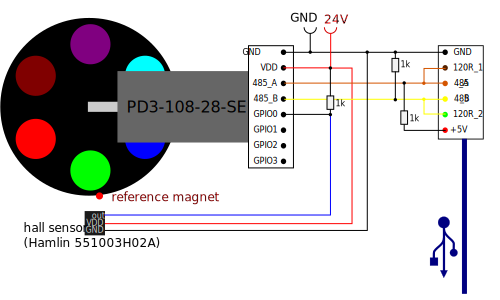
\includegraphics{schematic.pdf}
	\caption{Schematic of the control box PCB}
	\label{fig:schematic}
\end{figure}

\begin{figure}[H]
	\centering
		\includegraphics{pcb.pdf}
	\caption{PCB of the control box PCB}
	\label{fig:pcb}
\end{figure}

\begin{figure}[H]
	\centering
		\includegraphics{3dview.pdf}
	\caption{3D view of the control box PCB}
	\label{fig:3dview}
\end{figure}

\newpage
\subsection{Standard Operations Mode}
\label{sec:StandardOperationsMode}
The interface box will be in the so called standard operations mode (SOM) most of the time. In this mode the internal controller waits for any user interaction (either by the user interface elements (rotary encoder and buttons) or by the auxiliary I/O pins when in an external control mode) and sends the new settings to the laser controller if any change occurs. Several times each second this mode also acquires the laser status and displays it. Figure~\ref{fig:som_flowchart} shows a flowchart of this mode.

\begin{figure}[H]
	\centering
		\includegraphics{som_flowchart.pdf}
	\caption{Flowchart of standard operations mode}
	\label{fig:som_flowchart}
\end{figure}



\subsection{Implementation Details and Hints}
\label{sec:ImplementationDetailsAndHints}
\begin{itemize}
  \item The FTDI USB to serial converter has areprogrammed device name 
		\begin{center}
			\textit{LASERBOX}
		\end{center}
		Still you can use the standard FTDI virtual COM port driver for this device: 
		\begin{center}
			\url{http://www.ftdichip.com/FTDrivers.htm}
		\end{center}

	\item The FTDI USB to serial converter has to be programmed to be self-powered. Otherwise the serial connection does not work on Linux (on Windows system the problem does not seem to exist).
	\item You can bind a box to a spoecific serial port. On \textbf{Windows} this can be done in the driver settings. On \textbf{Linux} this may be achieved using the \texttt{udev} hardware enumeration system:
	
\begin{enumerate}
	\item create a udev rules file with a name like e.g.: \texttt{/etc/udev/rules.d/99-laserboxes.rules} 
	\item add a line like this:

{\footnotesize\begin{verbatim}
  #LASERBox
  KERNEL=="ttyUSB*", SUBSYSTEMS=="usb", ATTRS{product}=="B040SERVO", SYMLINK+="ttyUSB_B040SERVO" 
\end{verbatim}}

    which will map the ttyUSB device with the product name B040SERVO to the device file \texttt{/dev/ttyUSB\_B040SERVO} in addition to its default file \texttt{/dev/ttyUSB}\textit{x}. Instead of the product name you can also use any other USB device property, as reported by

{\footnotesize\begin{verbatim}
  lsusb -v -s <bus>:<devnum>
\end{verbatim}}

    Possible filters are e.g.:

{\footnotesize\begin{verbatim}
   ATTRS{serial}=="A800dOBl", 
   ATTRS{idVendor}=="1a72", 
   ATTRS{idProduct}=="1007", 
   ATTR{vendor}=="0x149a", 
   ATTR{device}=="0x0005"
\end{verbatim}}

    \item After saving the rules file you will have to tell udev that there are new/changed rules by executing

{\footnotesize\begin{verbatim}
  /etc/init.d/udev restart
\end{verbatim}}

    The rules will be executed when the new device is connected to the computer. So if it's already connected: pull and reconnect the plug.

\end{enumerate}
\end{itemize}




\subsection{Programming the Laserbox Controller}
\label{sec:ProgrammingTheLaserboxController}
The main microcontroller of the control box is an Atmel ATmega324p. It's flash memory may be programmed either by a standard AVR programmer, like usbasp (see \url{http://www.fischl.de/usbasp/} and Fig.~\ref{fig:usbasp}) or by a bootloader already installed on the controller. In the first case you should set the ``TargetSupply'' jumper of the usbasp and disconnect the power supply of the control box. This will supply 5V to the electronics of the control box which is OK for short periods (few minutes). Then you can use a programmer software like avrdude to program the controller. The programmer and the controller are connected by a standard $2\times3$ ribbon cable connectors (see Fig.~\ref{fig:3dview}).

If the controller is already equipped with the bootloader \texttt{avrprog\_boot v0.85} (by Martin Thomas, \url{http://www.siwawi.arubi.uni-kl.de/avr_projects#avrprog_boot}), you simply have to reset the controller (switch power off/on or use reset switch) while holding the ON/OFF button pressed down. Afterwards a new program can be loaded using a AVR109/AVR910 programmer software (e.g. avrdude, AVR Prog or AVR Studio) via the serial host port of the control box. Note that the bootloader is started only if the ON/OFF button is held down during a reset, otherwise the standard software starts and the control may be used to control a laser.

Here are some more hints on programming the controller:
\begin{itemize}
	\item The fuse bits for the ATmega324p controller without bootloader are: 
		\begin{center}
			\texttt{LFUSE = 0xFD;  HFUSE = 0xDF; EFUSE = 0xFF}.
		\end{center}
	\item The fuse bits for the ATmega324p controller with bootloader (2047 bytes) are: 
		\begin{center}
			\texttt{LFUSE = 0xFD;  HFUSE = 0xD8; EFUSE = 0xFF}.
		\end{center}
\end{itemize}


\begin{figure}[h]
	\centering
		\includegraphics[width=100mm]{usbasp.png}
	\caption{USBasp -- AVR programmer for USB}
	\label{fig:usbasp}
\end{figure}




\newpage
\section{Literature \& Datasheets}
\label{sec:literature_datasheets}
\begin{itemize}
  \item Cobolt Owners Manual, Version 04-01, Generation 4 Controller: \url{http://www.cobolt.se/docs/01-Owners Manual 0401 Gen 4 091201.pdf}
	\item ATmega324PV: \url{http://www.atmel.com/dyn/resources/prod_documents/doc8011.pdf}
  \item EA DOG-M 163: \url{http://www.lcd-module.de/pdf/doma/dog-m.pdf}
  \item LT1129-3.3: \url{http://cds.linear.com/docs/Datasheet/112935ff.pdf}
  \item FT232RL: \url{http://www.ftdichip.com/Documents/DataSheets/DS_FT232R.pdf}
  \item MAX3232: \url{http://datasheets.maxim-ic.com/en/ds/MAX3222-MAX3241.pdf}
  \item 74HCT164: \url{http://datasheets.maxim-ic.com/en/ds/MAX3222-MAX3241.pdf}
\end{itemize}
\end{document}

